\section{Cache performance nei sistemi paralleli/multicore}
Le performance della cache sono determinate da una combinazione del traffico dovuto ai singoli cache miss e al traffico dovuto alla comunicazione. I cache miss possono essere categorizzati (le 4 \textbf{c}):
\begin{itemize}
    \item \textbf{Conflict Misses}: misses che dipendono dal fatto che la cache non è full associative con LRU replacement;
    \item \textbf{Cold Misses}: Miss in quanto le cache all'avvio del sistema hanno tutti i blocchi invalidi;
    \item \textbf{Capacity Miss}: si verificano quando il \textit{working set} di un programma, ovvero l'insieme dei dati a cui esso accede in un determinato intervallo di tempo, eccede la capacità della cache;
    \item \textbf{Coherence Miss}: sono quei cache miss che non dipendono né dalla capacità della cache né dai conflitti di mappatura, ma dal fatto che in un sistema multiprocessore la coerenza della cache deve essere mantenuta. In pratica, un blocco che era già presente nella cache di un core può essere invalidato perché un altro core ha scritto in quella stessa linea di memoria. Quando poi il primo core torna ad accedere a quel blocco, non lo trova più valido nella sua cache e deve rileggerlo dal livello inferiore (o da un'altra cache): questo genera appunto un coherence miss.
\end{itemize}

\noindent Differenziamo inoltre i True e i False sharing misses: I True sharing misses sorgono dalla comunicaizone di dati attraverso il meccanismo di coerenza, e sono dovuti al fatto che uno stesso dato in memoria è condiviso e uno dei thread potrebbe invalidarlo causando un miss; i False sharing sorgono quando un core richiede una word pulita che si trova però in un blocco invalido. In altre parole sono i miss che accadono perchè la dimensione del blocco non è una sola word.

\begin{figure}[ht]
    \centering
    \setlength{\fboxrule}{0.5pt} % spessore sottile
    \setlength{\fboxsep}{0pt}    % senza spazio interno
    \fbox{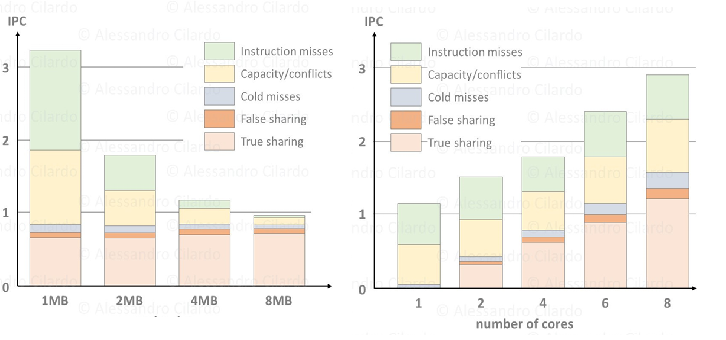
\includegraphics[width=0.8\textwidth]{fig/chapter_3/performances.png}}
\end{figure}